\chapter{Functional system overview}
This chapter goes into detail on the functional aspects of the myocardial perfusion phantom.
\section{Drivers}
\label{sec:drivers}
Many factors influence the outcome of \ac{MPI}. Some of these factors are:

\begin{tabular}{llll}
 	\multicolumn{1}{c}{\textbf{Tracer}} & \multicolumn{1}{c}{\textbf{Patient}} & \multicolumn{1}{c}{\textbf{Technology}} & \multicolumn{1}{c}{\textbf{Software}} \\
		- Concentration, & - Breathing artefacts, & - Modality, & - Package, \\
		- Volume, & - Cardiac motion, &  - Spatial resolution, & - Mathematical model, \\
		- Molecule size, & - BMI. & - Temporal resolution. & - Filters,\\
		- Injection speed.  & & & \makecell[l]{- \acs{ROI}.}\\
\end{tabular}

The strength of a phantom is that small modifications, for example, in contrast concentration or volume, or the mathematical model,  can be directly mapped to the outcome. It provides insight into dependent and independent factors in perfusion imaging.

Current phantoms either require modifications to software packages or do not model defects in a physiological way. Defects are typically modelled by reducing the flow through the myocardium by reducing the pump rate, effectively ignoring the complex relation between stenotic and non-stenotic arteries. Therefore, a myocardial perfusion phantom is needed that is compatible with clinical software and is able to mimic cardiac defects in a physiological way. This will increase the similarity with patient studies resulting in more reliable validation.

In addition to being a tool for validation of scanners and/or software packages, the phantom can be used for educational and training purposes to demonstrate the impact of hard- and software variables (sampling rate, \acf{ROI}, mathematical model), patient variables (BMI, blood flow and -pressure), tracer variables (concentration, type, injection speed), and many more.

\section{Approach}
The V-Model defines the project's development cycle. 

\subsection{Concept of operations}
\label{sec:concept_oper}
\subsection*{Is the D-SPECT's dynamic scanning, in comparison with other modalities (CT, MRI, PET, or SPECT), suitable for quantitative myocardial perfusion imaging?}
Quantitative flow measurements is made possible due to dynamic scanning. Dynamic scanning is not a newly emerged technique, it has been used with \ac{CT} in past research. Due to the solid-state detectors (Cadmium-Zinc Telluride), dynamic scanning is made possible for \ac{SPECT}. The D-SPECT is relatively new in the Netherlands. However, it has been employed in Japan, Canada, France, and Great-Britain. The D-SPECT is a highly specialised cardiac system. Due to the relatively small patient population, clinics often choose more all-purpose systems. The D-SPECT is very patient friendly due to its design in contrast to alternatives, e.g. GE uses a gantry design.

\ac{CT} is a well established modality with the highest spatial resolution. However, its largest drawback is that the radiation dose is directly proportional to the number of images, therefore increasing the likelihood of complication due to radiation exposure. \ac{MRI} does not rely an ionising radiation, but its lower temporal resolution makes it less suitable for dynamic imaging. \ac{SPECT} and \ac{PET} use radioactive tracers to image blood flow, thus exposing the patient to some degree of radiation. However, it is not directly proportional to the amount of images taken and is therefore less dangerous than \ac{CT}.

In addition, traditional \ac{SPECT} is, on average, 22\% less expensive than the current gold standard, \ac{PET}. D-SPECT is supposed to be even less expensive and faster. Furthermore, significant dose reduction, due to more sensitive solid-state detectors, reduces the strain and risk for patients. In addition, these solid-state detectors improve the image resolution. 

In summary, although the D-SPECT is relatively new in the Netherlands, it is more widely employed in Japan, Canada, France, and Great-Britain. The highly cardiac specialised system, its patient friendly design, the ability to scan faster and more accurate at significant dose reductions, make the D-SPECT suitable for quantitative myocardial perfusion imaging. 

\subsection{What must the myocardial perfusion phantom be able to simulate to validate quantitative MPI?}
\label{sec:what_perf}
The phantom must be compatible with clinical practice, i.e. use clinical protocols and hard-/software. Patients are scanned in a D-SPECT scanner while lying down, face up (supine). The scans are evaluated using 4DM software. 

The phantom must be suitable for an ROI in the left atrium for \ac{AIF} extraction. However, in case of poor results, the ROI can be reshaped and moved to the left ventricle. The software determines the perfusion in 17 areas of the left ventricle's myocardium, at a basal, mid and apical level, and at the apex. These segments are supplied via branches of the three coronary arteries, i.e. the RCA, LAD, and LCx. 4DM calculates individual flow rates for each segment. Therefore, the phantom should contain 17 segments where each segment is either static or with variable flow that can be measured. 

A single flow source is to be used that supplies the RCA, LAD, and LCx. From an anatomical viewpoint, the coronary arteries are supplied from the aorta. The phantom could mimic this anatomical structure, which is impractical. Instead, it is possible to supply the coronary arteries from a dedicated flow source significantly decreasing the total volume of liquid being displaced. Care must be taken such that the ratio of contrast remains equivalent. Since the entire myocardium is supplied by three coronary arteries, stenosis in one of the arteries, or its branches, results in different flow behaviour which cannot be mimicked by reducing the overall flow to the myocardium alone.

Every tracer behaves differently. For D-SPECT, Technetium (\textsuperscript{99m}Tc) Tetrofosmin is used. Only a small part of the total activity is absorbed by the myocardium; approximately 1.2\% in 5 minutes. Therefore, the uptake of tracer into tissue is not a necessity, it will be a design choice. 

\section{Business model}
\label{sec:bus_model}
Dynamic scanning yield quantitative results, i.e. absolute perfusion rates, which require proper validation. Phantom studies are, to a high degree, suitable for such purpose. An added benefit of these studies, is that it provides insight into the effect of different parameters on the outcome, which in turn influences patient treatment. These insights can be used for calibration or protocol optimisation, e.g. tracer protocol. Examples would be determining optimal (patient dependable) activity or injection speed.

In short, the phantom can be used for educational and training purposes, as well as for calibration or optimisation. 

The phantom will distinguish itself from other phantoms due to its more true-to-nature design, ability to physiologically mimic cardiac defects, and the possibility of modelling different compartment models.

The primary focus remains on the current application of \ac{MPI} as performed at the ZGT in Hengelo, Overijssel.

Please note, the phantom is developed during a master thesis to support the research of a PhD thesis. Therefore, there is no business plan to ensure profit, and to payback investments.

\section{Requirements}
\rrod{Verify the AIF requirements.}
The functional requirements are summarised in table \ref{tab:funcreq}.

\begin{table}[h]
\caption{Functional requirements}
\label{tab:funcreq}
This table summarises the functional requirements for the prototype myocardial perfusion phantom.
\begin{tabular}{l|p{120mm}|}
	\makecell[l]{Requirement \\ number} & \multicolumn{1}{c}{Description}\\
	\hline
	FR01 & The phantom must be able to simulate blood flow, either using water of blood-mimicking fluid, at high flow rates (aortic flow). \\ 
	\rowcolor{Gray}
	FR02 & The phantom must be able to simulate blood flow, either using water or blood-mimicking fluid, at low flow rates (myocardial flow). \\
	FR03* & An \ac{AIF} can be extracted from the left atrium, or alternatively from the left ventricle. \\
	\rowcolor{Gray}
	FR04 & Cardiac defects must simulate the complex relation between stenotic and non-stenotic arteries. \\
	FR05 & The phantom must be able to visualise (and measure) at least two active segments of the 17-segment ventricle model. \\
	\rowcolor{Gray}
	\sout{FR06} & \sout{The phantom must use a 2-compartment model (simulating contrast uptake in tissue).} \\
	FR07 & Tracer protocol must be equivalent to that used in clinical scans with D-SPECT. \\
	\rowcolor{Gray}
	\sout{FR08} & \sout{Contrast should be mixed equivalently to contrast mixing in patients.} \\
	\cline{2-2}
\end{tabular}
\raggedright
\textit{* Depending on the flexibility of the clinical software.}
\end{table}

\section{Business and system use cases}	
The myocardial perfusion phantom is used by researchers with varying goals. Primarily, the phantom set-up is a tool to validate perfusion imaging hard- and software and to educate on independent and dependent factors, see section \ref{sec:drivers}. The researcher should be able to adjust the blood flow, both in the myocardium and in the aorta, and be able to set a cardiac defect.

Please note, setting the imaging and contrast parameters are not part of the phantom itself. 
\begin{figure}[!h]
	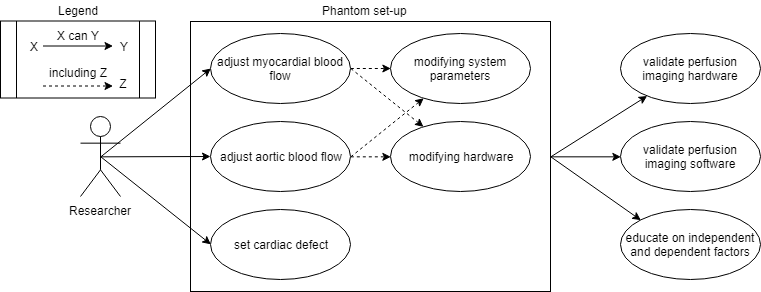
\includegraphics[width=\textwidth]{./images/usecase_diagram.png}
	\caption{Use case diagram for the prototype myocardial perfusion phantom}
	\label{fig:usecase}
\end{figure}

\section{Architectural overview}
A schematic overview of the flow set-up is shown in figure \ref{fig:funcarch}. The set-up consists of a flow generating system, e.g. mechanical pumps or pressure based, to generate the required aortic and myocardial flow, measuring systems, e.g. flow and pressure sensors, and the phantom itself, simulating the heart. The flow is controlled by means of a control system, over which the user has control. The flow parameters, i.e. flow and pressure, are measured by sensors which are monitored by a monitoring system. The monitoring system and control system cooperate such that user parameters are maintained. Figure \ref{fig:funcarch} shows a distinction between high and low flow, which is not a requirement. Low flow can be created by means of pressure difference in high and low flow circuit; increasing pressure in low flow circuit results in less volume passing through.
\begin{figure}
	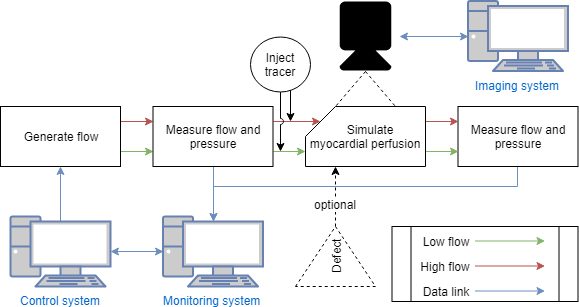
\includegraphics[width=0.75\textwidth]{./images/functional_architecture.png}
	\caption{Functional architecture for the myocardial perfusion set-up. The myocardial perfusion is simulated in normal situations and in defect situations. The manner in which a defect situation is simulated, is a design choice. \textbf{Figure for indicative purposes, subject to change}.}
	\label{fig:funcarch}
\end{figure}
